\section{Datensätze}

In diesem Abschnitt wird der in dieser Arbeit verwendete Datensatz sowie dessen grundlegende Eigenschaften beschrieben. Sämtliche in der Masterarbeit eingesetzten Bild- und Videodaten stammen aus der öffentlich zugänglichen \textit{Mosquito Breeding Grounds V2 (MBG-V2) Database}, die von der Federal University of Rio de Janeiro (UFRJ) bereitgestellt wird. Der Datensatz wurde in der Stadt Rio de Janeiro, Brasilien, mithilfe von Drohnenplattformen aufgezeichnet und umfasst Videoaufnahmen urbaner Gebiete, die ein erhöhtes Risiko für die Bildung von Mückenbrutstätten aufweisen.

Die MBG-V2-Datenbank besteht aus hochauflösenden Drohnenvideos, die unter unterschiedlichen Umweltbedingungen, aus variierenden Flughöhen sowie mit wechselnden Kamerabewegungen aufgenommen wurden. In den Videoaufnahmen sind unter anderem offene Wasseransammlungen, Behälter, Abfallbereiche und weitere potenzielle Brutstätten für Stechmücken in städtischen Umgebungen zu sehen. Diese Vielfalt an Szenarien und Bildinhalten macht den Datensatz besonders geeignet für videobasierte Objekterkennungs- und Analyseaufgaben.

\subsection{Mosquito Breeding Grounds V2 (MBG-V2) Database}

In dieser Arbeit wird die \textit{Mosquito Breeding Grounds V2 (MBG-V2) Database} verwendet, die von der Federal University of Rio de Janeiro (UFRJ) veröffentlicht wurde \cite{passos2024mbgv2}. Die MBG-V2-Datenbank stellt die zweite Version eines annotierten, video-basierten Drohnendatensatzes dar, der speziell für die Detektion potenzieller Brutstätten der Stechmücke \textit{Aedes aegypti} in urbanen Umgebungen entwickelt wurde. Im Vergleich zur ersten Version umfasst MBG-V2 eine größere Anzahl an Videosequenzen, die ausschließlich unter realen Einsatzbedingungen aufgenommen wurden, sowie eine erweiterte Anzahl an Objektklassen. Dadurch stellt der Datensatz eine realistischere und zugleich anspruchsvollere Grundlage für computer-vision-basierte Analysen dar.

Die Videoaufnahmen wurden mithilfe eines unbemannten Luftfahrzeugs (Unmanned Aerial Vehicle, UAV) mit hochauflösender Kamera in der Stadt Rio de Janeiro, Brasilien, durchgeführt. Insgesamt wurden 13 unterschiedliche urbane Regionen überflogen. Aufgrund von Dateigrößenbeschränkungen wurde jede Region in zwei komplementäre Videosequenzen unterteilt, sodass der Datensatz insgesamt 26 Videos umfasst. Alle Flüge wurden in einer konstanten Flughöhe von etwa 40 Metern durchgeführt.

Wie in Abbildung~\ref{fig:mbgv2_regions} dargestellt, sind die überflogenen Regionen (A--M) innerhalb des Stadtgebiets von Rio de Janeiro verteilt und repräsentieren unterschiedliche urbane Strukturen.

\begin{figure}[H]
    \centering
    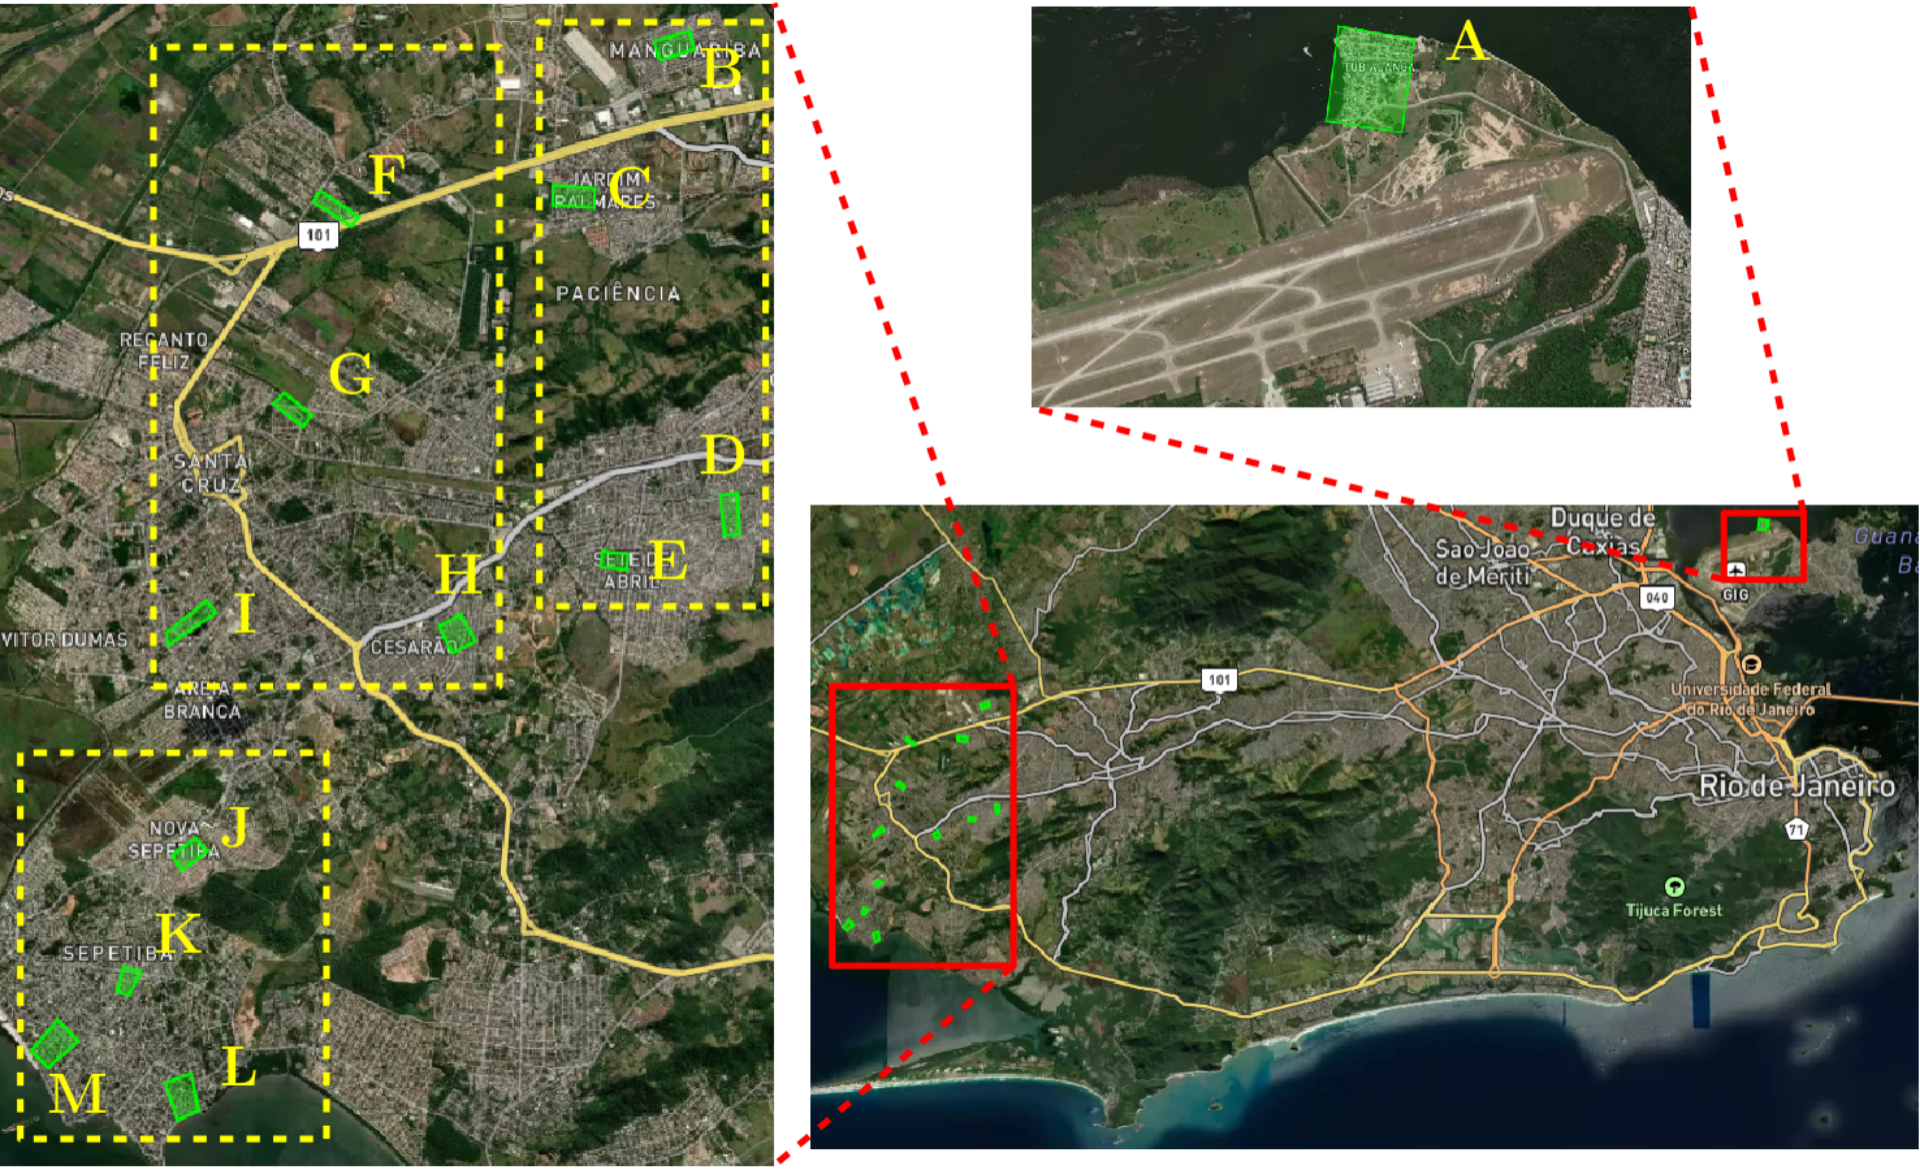
\includegraphics[width=0.9\linewidth]{figures/datasets/rio_areas.png}
    \caption{Lage der überflogenen MBG-V2-Regionen (A--M) innerhalb der Stadt Rio de Janeiro.}
    \label{fig:mbgv2_regions}
\end{figure}

Zur systematischen Erfassung der Zielgebiete wurde ein serpentinenförmiges Flugmuster eingesetzt, das eine gleichmäßige und vollständige Abdeckung der ausgewählten Areale ermöglicht.

Abbildung~\ref{fig:mbgv2_flightpattern} zeigt exemplarisch das dabei verwendete Flugmuster.

\begin{figure}[H]
    \centering
    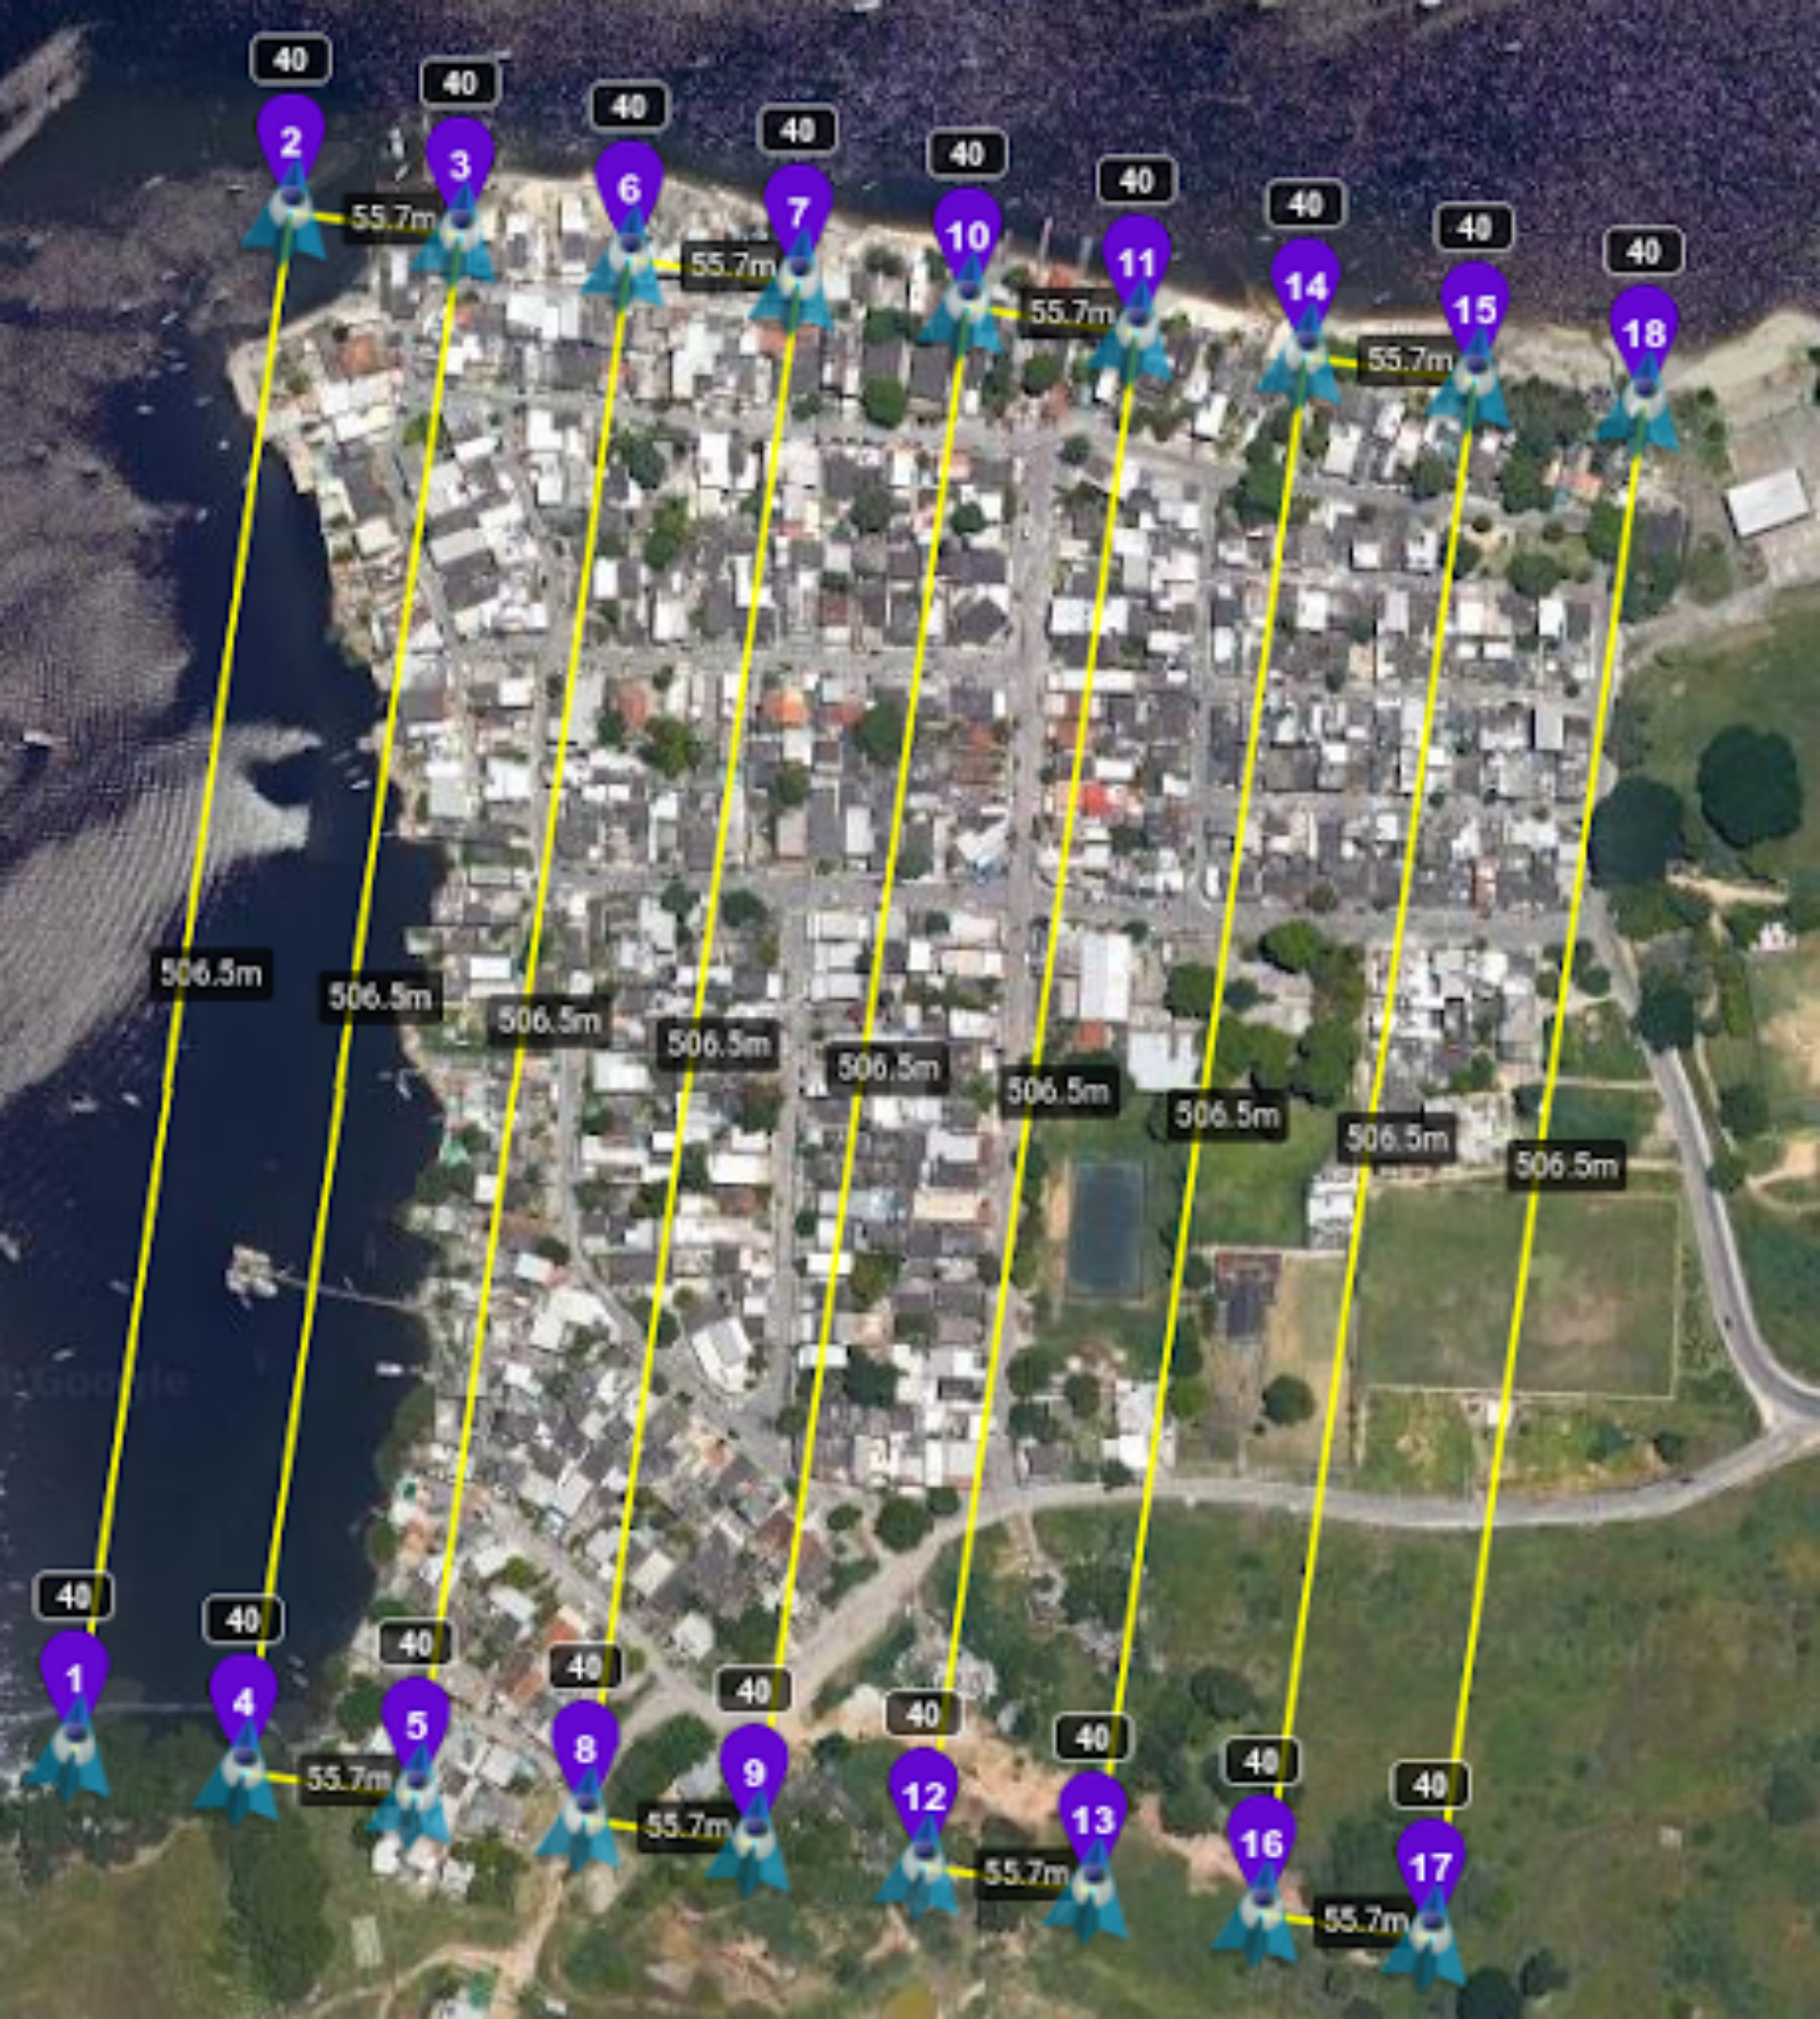
\includegraphics[width=0.6\linewidth]{figures/datasets/flight_planning.png}
    \caption{Serpentinenförmiges Flugmuster zur systematischen Datenerfassung im MBG-V2-Datensatz.}
    \label{fig:mbgv2_flightpattern}
\end{figure}

Die MBG-V2-Datenbank enthält Annotationen für mehrere Objektklassen, die als potenzielle Brutstätten von \textit{Aedes aegypti} gelten. Dazu zählen unter anderem Flaschen, Eimer, Pools, Wasserpfützen, Reifen, Wassertanks, Müllcontainer, große und kleine Abfallbehälter, Plastiktüten, Topfpflanzen sowie Straßeneinläufe. Die Annotationen liegen in Form von Bounding-Box-Markierungen vor und wurden im XML-Format des \textit{Computer Vision Annotation Tool} (CVAT) erstellt \cite{cvat2024}. Dieses Format unterstützt track-basierte Annotationen, sodass Objekte über mehrere aufeinanderfolgende Videoframes hinweg konsistent beschrieben werden können.

Zusätzlich zu den Videodaten stellt die MBG-V2-Datenbank ergänzende Metadaten zur Verfügung. Dazu gehören Flugprotokolle mit Telemetriedaten des UAVs, wie unter anderem Lageparameter und Geschwindigkeit, sowie geographische Informationen zu den Grenzen der erfassten Regionen. Diese Zusatzinformationen ermöglichen eine weiterführende zeitliche und räumliche Analyse der aufgezeichneten Daten.



\subsection{Verwendung des MBG-V2-Datensatzes in dieser Arbeit}

Im Rahmen dieser Arbeit wurde der Mosquito Breeding Grounds V2 (MBG-V2) Datensatz nicht unverändert verwendet, sondern gezielt an die Anforderungen der vorliegenden Untersuchung angepasst. Da es sich bei MBG-V2 um einen video-basierten Datensatz handelt, wurden die Videosequenzen zunächst in einzelne Bildframes zerlegt. Dieser Schritt ermöglicht die Anwendung bildbasierter Annotations- und Analyseverfahren in den nachfolgenden Verarbeitungsschritten.

Die im MBG-V2-Datensatz bereitgestellten Annotationen liegen im XML-Format des Computer Vision Annotation Tool (CVAT) vor und sind track-basiert organisiert \cite{cvat2024}. In dieser Arbeit wurden aus den Videosequenzen lediglich ausgewählte Frames manuell annotiert. Konkret wurde ungefähr jedes 30. Frame eines Videos für die manuelle Annotation herangezogen, während die dazwischenliegenden Frames zunächst unannotiert blieben. Dieses Vorgehen zielt darauf ab, den manuellen Annotierungsaufwand zu reduzieren und gleichzeitig die Grundlage für die Evaluation halbüberwachter Methoden zu schaffen.

Bei den manuell annotierten Frames wurden die im MBG-V2-Datensatz definierten Objektklassen unverändert übernommen. Diese Klassen repräsentieren Umweltobjekte, die als potenzielle Brutstätten von \textit{Aedes aegypti} gelten. Die Annotationen wurden in Form von Bounding-Box-Markierungen vorgenommen, um die räumliche Lage der Objekte innerhalb der Bildframes eindeutig zu erfassen.

Die im CVAT-Format vorliegenden Annotationen wurden anschließend in ein für die in dieser Arbeit eingesetzten Objekterkennungsmodelle geeignetes Format überführt. Hierbei wurden die track-basierten Annotationen in framebasierte Labels umgewandelt, sodass für jedes Bild die zugehörigen Klasseninformationen und Bounding-Box-Koordinaten vorlagen. Auf diese Weise wurde der MBG-V2-Datensatz für die Durchführung bildbasierter automatischer Annotations- und Objekterkennungsverfahren vorbereitet.

Der in diesem Abschnitt beschriebene Datenaufbereitungsprozess bildet die Grundlage für die im weiteren Verlauf der Arbeit vorgestellten Methoden zur automatischen Annotation und halbüberwachten Modellanpassung.
